\chapter{Loaded elastic beam}

\modinfo{Directory}{ElasticBeam}

\section{Solution with linear model} 


\modinfo{Solvers}{\Idx{StressSolve}}
\modinfo{Tools}{\Idx{ElmerFront}}
\modinfo{Dimensions}{2D, Steady-state}

\subsection*{Case definition}

A homogenous, elastic beam ($\Omega$) is rigidly supported on one 
end (boundary $\Gamma_4$). On boundary $\Gamma_3$ the beam is subjected 
to a load $q(x)$, which grows linearly from zero to $q_0$ 
(see figure~\ref{fg:beam}). Material properties of the beam are the Poisson 
ratio 0.3 and Young's modulus $200\cdot 10^9$N/m$^2$. Problem is to solve the 
displacement of the beam.  

\begin{figure}[h]
\centering
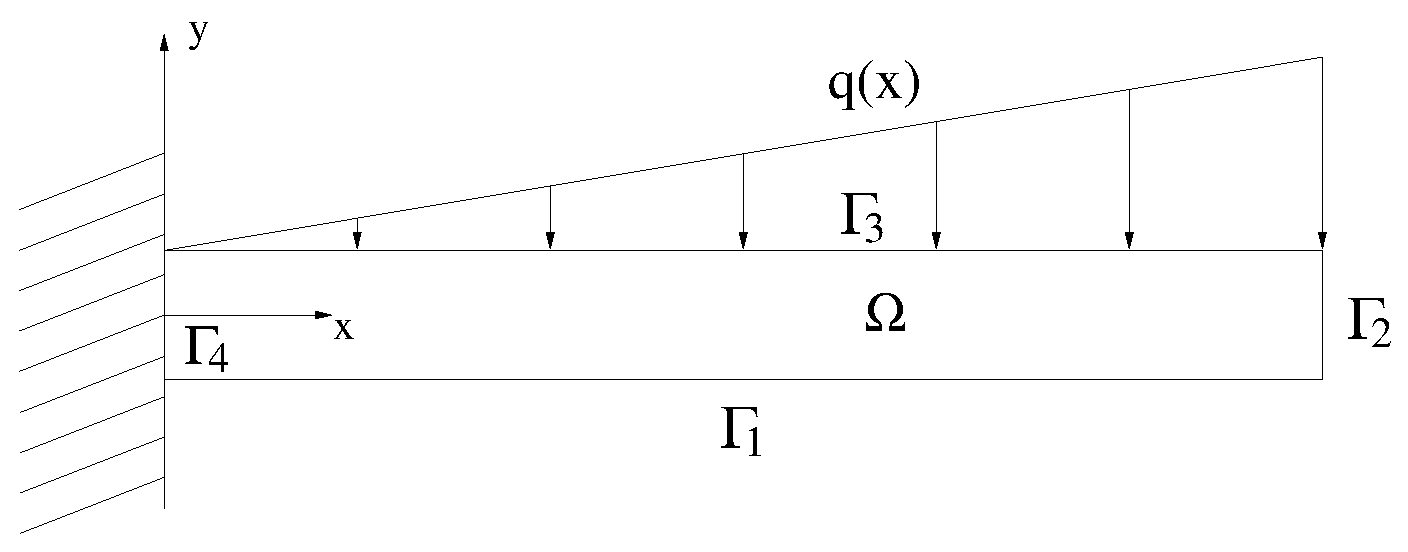
\includegraphics[width=100mm]{Beam}
\caption{Beam and loading.}\label{fg:beam}
\end{figure}

Problem is solved according to linear elasticity theory. Mathematically 
the problem to be solved is
\begin{equation}
\left \{
\begin{array}{rcll}
-div \sigma & = & 0 & \mbox{ in } \Omega \\
\sigma & = & \lambda tr [\varepsilon(u)]I + 2 \mu \varepsilon(u) &
\mbox{ in } \Omega \\
u & = & 0 & \mbox{ on } \Gamma_4 \\
\sigma n & = & 0 & \mbox{ on } \Gamma_1 \cup \Gamma_2 \\
\sigma n & = & -q & \mbox{ on } \Gamma_3 \\
\end{array}
\right .
\end{equation}
where $\lambda$ and $\mu$ are the Lam\'{e} constants (which can be expressed 
in terms of the Poisson ratio and Young's modulus), $\varepsilon$ is the 
linearized strain tensor, $u$ is the displacement vector, $q$ is the given
surface traction and $n$ is the outward unit normal to the boundary.

\subsection*{Solution procedure}

\begin{itemize}
\item Start ElmerFront.
\item Open the file that contains the geometry of the beam from 
the File menu. Select also the working directory for the model.
\ttbegin
File -> Open cad-file 
  File = Beam.egf 
  Model name = Beam 
  Model directory = beam_tutorial
\ttend
\item Select the equations to be solved from the Problem menu. In this 
case stress analysis is selected. It solves the problem according to 
linear elastic theory. 
\ttbegin
Problem -> Equations 
  Stress analysis 
\ttend
\item Define the material properties from the Model menu. Give the values for 
Young's modulus and the Poisson ratio. Add the defined material 
properties to the material property sets so they become attached 
to $\Omega$. 
\ttbegin
Model -> Materials 
  Young's modulus = 200e9 
  Poisson ratio = 0.3
\ttend

\item Define the Dirichlet boundary condition and the load from the
Model menu. Give the value zero for displacements at the boundary
$\Gamma_4$ and press Add. The linearly varying load is defined in the
same panel as follows.  Select the boundary~3, click the cursor on to
the Force-y line, check the box Table, and press finally the Edit
button. A window opens in which the tabular bc entry is
defined. Select first Coordinate 1 as the variable on which the
Force-y depends. Write on the line below entry {\tt 0 0}. Click
Add. Write {\tt 1 -1.0e7} on the line and click again Add. Now, the
space below contains two lines written in two columns. The first
colums holds the values for the Coordinate~1 and the second column for
the Force-y. The value of the force is interpolated according to these
definitions. Now click OK on the Table entry panel. In Boundary
Conditions panel, click Add and then OK.
\ttbegin
Model -> Boundary conditions
Boundary 4
Displacement-X = 0
Displacement-Y = 0
Add
Boundary 3
Force-Y
Table
Edit
Variable = Coordinate 1
0 0
Add
1 -1e7
Add
OK
Add
OK
\ttend

\item Define mesh from the Mesh menu. First give name for the
mesh. Then select ``Mesh structure'' and define element type and the
number of elements. Attach the defined mesh structure to the Body~1
and click OK. Create the mesh by pressing ``Generate mesh'' button.

\ttbegin 
Mesh -> Define mesh 
Mesh name = Mesh1 
Mesh structure 
Element type = Quad 
Nof elements (1st and 3rd edge) = 40 
Nof elements (2nd and 4th edge) = 4 
Add 
OK 
Generate mesh 
\ttend
\item Now to solve the problem defined with the constant load select from 
the Run menu item Solver. 
\ttbegin
Run -> Solver 
\ttend
\item Results may be viewed with the ElmerPost program
\ttbegin
Run -> Postprocessor
\ttend
or click the {\tt Results} button on the main window.
\end{itemize}

\subsection*{Results}

As a result the absolute value of maximum displacement is given. The 
displacements calculated with different load values $q_0$ are tabulated in 
table~\ref{tb:struct3a}. Note that the absolute value of the
displacement varies linearly with respect to the load since the model
is linear.

\begin{figure}[h!]
\begin{center}
  \includegraphics[width=0.30\textwidth,angle=0]{respic1.png}
  \includegraphics[width=0.28\textwidth,angle=0]{respic2.png}
  \includegraphics[width=0.25\textwidth,angle=0]{respic3.png}
  \caption{The displacement of an elastic beam with different loads
using a linear model}
  \label{fig:elast_beam1}
\end{center}
\end{figure}

\begin{table}[h]
\caption{Displacements with different load values}
\label{tb:struct3a}
\begin{center}
\begin{tabular}{ll} \hline
$q_0$ [N/m$^2$] & $\max |u|$ [m] \\ \hline
-1.0$e7$ & 0.04862 \\
-1.0$e8$ & 0.4862 \\
-1.0$e9$ & 4.862 \\ \hline
\end{tabular}
\end{center}
\end{table}

If you look at the results you can see that the displacement values
become relatively large. The linear theory is valid only to small 
displacements. From Fig~\ref{fig:elast_beam1} you can also notice that the
beam does not maintain its original form. This means that the linear 
elasticity theory can not take into consideration all the necessary 
phenomenona that are related to the problem, anymore. To be able to 
solve the problem we must use general elasticity theory. This is done 
in the following subsection.


\section{Solution with nonlinear model}

\modinfo{Solvers}{\Idx{ElasticSolve}}
\modinfo{Tools}{editor}
\modinfo{Dimensions}{2D, Steady-state}

\subsection*{Case definition}

In the following the beam problem is solved with general elasticity theory.
That is done by using the nonlinear elasticity solver of Elmer. 
In the case of homogenous 
elastic material the problem can be written into a following mathematical form

\begin{equation}
\left \{
\begin{array}{rcll}
-div [(I+ \nabla u) \Sigma] & = & 0 & \mbox{ in } \Omega \nonumber \\
\Sigma & = & \lambda (tr E)I + 2 \mu E & \mbox{ in } \Omega \nonumber \\
E & = & \frac{1}{2}(\nabla u^{T} + \nabla u + \nabla u^{T} \nabla u) & 
\mbox{ in } \Omega \nonumber \\
u & = & 0 & \mbox{ on } \Gamma_4 \\
(I+ \nabla u)\Sigma n & = & 0 & \mbox{ on } \Gamma_1 \cup \Gamma_2 \\
(I+ \nabla u)\Sigma n & = & -q & \mbox{ on } \Gamma_3 \\
\end{array}
\right .
\end{equation}
where $u$ is the displacement vector, $q$ is the given surface load, $\Sigma$ 
is the second Piola-Kirchhoff stress tensor, $\lambda$ and $\mu$ are the 
Lam\'{e} constants and $E$ is the Green-St Venant strain tensor.


\subsection*{Solution procedure}

The problem is solved here without the graphical user interface.
Open the solver input file of the linear case, Beam.sif, and edit the
following changes. Define nonlinear elasticity as the only equation
\ttbegin
Equation 1
  Name = "Equation1"
  Nonlinear Elasticity = Logical True
End
\ttend

Change the name correspondingly in the Solver block and add
information about the procedure needed. Leave all other keywords on
the solver block unchanged.
\ttbegin
Solver 1
  Equation = "Nonlinear Elasticity"
  Procedure = "ElasticSolve" "ElasticSolver"
...
End
\ttend

Finally, the force load may be changed in boundary condition 2 as
\ttbegin
  Force 2 = Variable Coordinate 1
      0 0
      1 -1.0000e+09
    End
\ttend

The problem may now be solved from the command line by typing {\tt
ElmerSolver}.

\subsection*{Results}

\begin{table}[tbhp]
\caption{Maximum displacements with different load values calculated according to 
general elasticity theory and linear theory.}
\label{tb:struct3b}
\begin{center}
\begin{tabular}{lll} \hline
$q_0$ [N/m$^2$] & 
$\max |u|$ [m] &
$\max |u|$ (linear) [m] \\ \hline
-1.0e$^7$ & 0.04890 & 0.04862 \\
-1.0e$^8$ & 0.4532 & 0.4862  \\
-1.0e$^9$ & 1.297  & 4.861 \\ \hline
\end{tabular}
\end{center}
\end{table}

From table~\ref{tb:struct3b} you can see the difference between the 
results calculated according to nonlinear and linear theory. According to 
the linear theory the displacement increases linearly as the load 
increases. This can be seen clearly from the results. The last loading
level (-1.0e9 N/m$^2$) is fairly large and the beam would probably break 
under that load. So the value of displacement might be unrealistic in that
case.   


\vfill
\mbox{}
